%------------------------------------------------------------------------------
% This is a LaTeX template for the scientific justification of IRAM Proposals 
%------------------------------------------------------------------------------
% 
% We encourage IRAM proposers to use this template for the sake of unity 
% and clarity when Program Committee members assess their proposals.
% 
% You may customize this template to suit your preferences (e.g. using BibTex),
% but please respect the following requirements:
%     The scientific justification should contain a maximum of 2 pages of text 
%     (4 pages for Large Programs), plus 2 pages of Figs., Tables and Refs.
%     The font size should be 11pt or larger.
%
% For Large Programs, the following sections should be included: 
%   i) Scientific Rationale, 
%  ii) Immediate Objective, 
% iii) Feasibility and Technical Justification, and 
%  iv) Organizational Issues.
% 
%
%------------------------------------------------------------------------------
%
\documentclass[11pt,a4paper,twoside,graphicx,color]{article}
%
\usepackage[margin=2cm]{geometry}
\usepackage[pdftex]{graphicx}
\usepackage{color}
\usepackage{txfonts}
\usepackage{paralist}
\usepackage[numbers]{natbib}
\setlength{\bibsep}{0.0pt}
\usepackage{amssymb}

\newcommand{\ccor}[1]{\textcolor{red}{#1}}

\bibpunct{(}{)}{;}{a}{}{,} % to follow the A&A style
\bibliographystyle{aa} % style aa.bst

%
% Page size and text dimensions
% Do not change!
\textheight 260mm
\textwidth 178mm
\oddsidemargin -8mm
\evensidemargin -8mm
\marginparwidth 50pt
\topmargin -22mm
\brokenpenalty=10000
\sloppy
%
%-------------------------------------------------------------------
\begin{document}
%
%
\begin{center}{\huge \bf
%-------------------------------------------------------------------
High resolution observations of the thermal tSZ effect from galaxy clusters
%-------------------------------------------------------------------
}\end{center}
% 
\begin{center}
{\bf NIKA2 Guaranteed Time Large Program}

{\bf 300 h of allocated time}
\end{center}

\begin{center}
J. F. Mac\'ias-P\'erez (LPSC), E. Pointecouteau (IRAP), B. Comis (LPSC), R. Adam (LPSC), N. Aghanim (IAS), M. Arnaud (CEA), F.X. D\'esert (IPAG), M. Douspis (IAS), F. Mayet (LPSC), J. B. Melin (CEA), L. Perotto (LPSC), G. Pratt (CEA), J. A. Rubi\~no-Mart\'in (IAC), F. Ruppin (LPSC)
\end{center}

%-------------------------------------------------------------------
\vspace{-0.3cm}
%\section{Scientific context}
%\vspace{-0.3cm}
{\bf \Large Abstract -- } 
We describe here the NIKA2 Guaranteed Time Large Program dedicated to high resolution observations of clusters of galaxies at intermediate and high redshift via the thermal Sunyaev-Zeldovich (tSZ) effect, for a total of 300 hours. %NIKA2 is well adapted for high angular resolution follow-up observations because of its large number of high sensitive detectors observing at two frequency bands (150 and 260 GHz), its large field of view (6.5 arcmin) and the resolution allowed by a 30 m telescope (17.5 and 11 arcsec, respectively at the two frequencies). 
We intend to observe a large sample of clusters (50 objects in total) representative of the cluster population in the redshift range from 0.5 to 1.5, for which the FOV and resolution of NIKA2 are particularly well adapted. The main output of the program will be: i) the study of the redshift evolution of the cluster pressure profile and of the scaling laws relating cluster observational properties (i.e. the integrated Compton parameter and the cluster total masses), ii) the study of the dispersion of the cluster population around its average behaviour and its correlation with the morphology and dynamical state of the objects (at z $>$ 0.5). This will be achieved through NIKA2 sub-arcminute resolution tSZ observations, leading to major improvements on the use of clusters of galaxies to draw cosmological constraints.\\

\vspace{-0.1cm} \noindent {\bf \Large Scientific context -- }
As the largest gravitationally collapsed objects in the universe, clusters of galaxies represent the last step of the hierarchical gravitational process of structure formation. Therefore their abundance in mass and redshift is strongly related to the power spectrum of the primordial density fluctuations, to the cosmological parameters and their evolution all along the history of our Universe. 

Most of the cluster baryons are present as a diffuse gas, the Intra-Cluster Medium (ICM), hot (10$^6$ - 10$^8$ K) and completely ionized. 
Due to its physical state, the ICM is responsible for a secondary anisotropy of the Cosmic Microwave Background (CMB): the thermal Sunyaev-Zel'dovich (tSZ) effect. Through their path toward us, CMB photons may interact with the free hot electrons in the ICM, being then shifter to higher energies. This results in a CMB flux decrement (increment) at frequencies below (above) 217 GHz, which corresponds to a distortion of the CMB spectrum. The amplitude of the effect is proportional to the integral of the pressure of the electron population along the line of sight (y~$\propto \int P_{e} dl$). Measuring the  distribution of the tSZ signal in clusters directly probes the distribution of thermal pressure within the ICM. Furthermore, being a CMB spectral distortion, the tSZ flux is not affected by redshift cosmic dilution. Thus, the tSZ effect represents an interesting observable to detect and study clusters at high redshifts, where their number and distribution is the most sensitive to the underlying cosmology \citep[e.g.][]{Carlstrom2002}.

In the last few years, technological progresses have made possible to detect the tSZ effect routinely. As a consequence, tSZ-selected cluster catalogues containing several thousands of candidates have finally been produced, at arcmin resolution, by the South Pole Telescope \citep[SPT, FWHM $\sim$ 1.1 arcmin at 150 GHz,][]{Reichardt2013, Bleem2014}, the Atacama Cosmology Telescope \citep[ACT, FWHM $\sim$ 1.4 arcmin at 148 GHz, ][]{Hasselfield2013}, the Planck satellite \citep[FWHM $\sim$ 10 arcmin for tSZ,][]{PSZ1, PSZ2}.  
ICM observables, such as the tSZ flux, can provide a valuable tool for cosmological investigation with clusters, as long as we are able to convert them into robust mass estimates. In fact, at present, the systematic uncertainties affecting the observable to mass relations represent the limit for cluster-derived cosmological constraints. Planck, ACT and SPT have detected many clusters through tSZ performing a blind survey able to use this effect to identify objects not yet discovered at other wavelengths. However, their relatively limited resolution ($\gtrsim$ 1 arcmin) only allows detailed study of the spatial distribution of the signal for low redshift clusters. However, the use of tSZ-selected cluster samples for cosmological purposes also requires an accurate understanding of the astrophysical systematics affecting the baryonic proxies (i.e. the tSZ integrated flux, $Y$) of the cluster total mass (M$_{tot}$), even at high-z. In this context, {\bf measurements reaching sub-arcminute angular resolution for cluster pressure profiles are a mandatory step for precise cluster and tSZ cosmology, since they will contribute to improve our knowledge of the statistical properties of galaxy cluster structure reducing the related uncertainties and biases, which now limit cosmological studies} \citep[e.g.][]{number_counts2015, ymap}. 
%Clusters grow by constant smooth accretion and violent merger events. This mechanism driving the growth of structures impacts cluster content, and thereby this complex accretion history imprints
%the energy distribution within the ICM. Furthermore, feedback from galaxy formation (through AGN and SFR/SN) also impacts the properties of the gas, injecting energy within the ICM which is known to counterbalance the gravitational radiative cooling of the hot gas. These energy injections modify the thermodynamical state of the ICM and then they might also affect its observable properties, in a way that must be quantified.

Such measurements can only be made possible by high sensitivity and high spatial resolution tSZ observations. 
The NIKA2 camera at the IRAM 30~m telescope is a well-suited instrument for this kind of observations and follow-ups, given its resolution, sensitivity and dual-band observation capability (as it will be detailed later). Conducting sub-arcminute tSZ observations of a representative population of clusters across a large redshift range will bring detailed insight of the properties of clusters over more than 3 Gyr. This will allow us to understand the processes driving the physical evolution of massive halos in the universe and to quantify 
%how cluster properties evolve with time. %The investigation of the physical state of groups and clusters as a function of redshift will thus help us to asses the evolution involved by the cluster accretion history, the processes at play in a gravitationally bound system and spread light on the co-evolution of the different  cluster baryonic components (i.e. the hot intra-cluster gas and the cluster galaxies). 
%Indeed studies across a large and representative population of high redshift
%clusters will permit to quantify the evolution of 
how the cluster thermal content and distribution evolves as massive
halos continue to grow through accretion and merging processes. 

%\vspace{0.3cm} \noindent {\bf \Large NIKA2 tSZ large program  -- }  \\

\vspace{0.3cm} \noindent {\bf \Large Objectives and main foreseen outpus -- } 
\\
The main objective of this program is to obtain {\bf high resolution} tSZ observations for a sample of objects, which are {\bf representative} of the population of clusters of galaxies, at {\bf intermediate and high redshifts (z $>$ 0.5)} and spanning more that an order of magnitude in Y$_{500}$ (and then also in M$_{500}$). These observations will be used for an in-depth study the evolution of cluster physical properties across cosmic times. At present, cluster and tSZ derived cosmological constraints are limited by our incomplete understanding of the impact of the details of cluster astrophysics. Thus, this study is mandatory to handle systematics and achieve precision cosmology with clusters. 
%As discussed before, NIKA2 is well adapted to explore the cluster population at intermediate and high redshift, within r$_{500}$ (self-similar scale).%and at r $>$ r$_{500}$ (non-equilibrium regions).
%
%We aim at characterizing the details of the tSZ signal distribution in clusters at z~$>$~0.5,  The complementary information provided by the NIKA2 follow-up will lead to better understand and quantify the systematic uncertainties that might affect blind tSZ surveys (such as detection biases, constraining typical SZ profiles). 
More precisely we aim at:
\begin{itemize}
	\item [-] Exploring and test the regularity of the cluster pressure profile at z~$>$~0.5, reproducing what has been done with the REXCESS sample at z~$<$~0.2 \citep{Arnaud2010}, but with an observable (the SZ signal) that probes directly the ICM pressure. Is still pressure the quantity less affected by the cluster dynamical state and thermodynamic history, event high-z? 
	\item [-] Detecting the presence of sub-structures (e.g. secondary peaks, deviations from spherical symmetry, overall irregular shape) and their significance. 
	\item [-] Introduce, define and test parameters that allow us to quantify the cluster dynamical state through its tSZ morphology. A robust tSZ-defined indicator of cluster morphology would permit to study the disturbed cluster fraction as a function of redshift and would represent a useful tool to explore its correlation with deviation from the self-similar behavior (for both the pressure profile and scaling laws).
	\item [-] Study the correlation between the SZ indicator(s) of cluster dynamical state and the dispersion around the average cluster pressure profile. Does the dispersion increase with redshift? Is it the same at any radial scale?
\end{itemize} 

\vspace{0.3cm} \noindent {\bf \large Target selection-- } \\
Our target selection strategy is mainly driven by the need of selecting {\bf a sample of objects which is representative of the cluster population}.
A flux selected subset of an tSZ-selected catalogue can be considered as representative of a sample that is not biased towards a given morphology.  {\bf We want to derive relations that can be applicable to the whole cluster population} (not only relaxed or un-relaxed) {\bf in order to achieve a good global characterization of clusters and an improved control of systematics due to their astrophysics}.
This criterion follows in fact the approach adopted to build the REXCESS sample \citep{REXCESS}, an XMM-Newton large program dedicated to the in-depth study of a representative sample of 33 clusters (0.055 $<$ z $<$ 0.183). This sample has in fact been used to build the universal pressure profile for the ICM \citep[][ an average profile for the cluster population, derived from observations, scaled by mass and redshift according to the standard self-similar model]{Arnaud2010}. 

In order to fulfill our goal with NIKA2, we consider the following main target selection criteria:
\begin{itemize}
  \item [-] clusters belonging to tSZ selected samples (already existing tSZ based cluster samples from Planck and ACT), for which the redshift information is available;
  \item [-] z $>$ 0.5, going up to to 1.5, to explore the cluster statistical properties beyond the local Universe;
  \item [-] dec $>$ -11, to ensure observability of the sources from the Pico Veleta site.
\end{itemize}

The number of objects fulfilling these requirement are provided in Tab. \ref{tab:availables}. 
The right panel of Fig. \ref{Fig:CL_and_sample} shows those objects in the z~-~Y$_{500}$ plane.


\begin{table}
\centering
\begin{tabular}{|l  || c | c | c || c |}           
 \hline    
  &  0.5 $\leq$ z $<$ 0.7  & 0.7 $\leq$ z $<$ 0.9 & 0.9 $\leq$ z $<$ 1.1 & no z available\\ \hline
  PSZ1 & 40 & 11 & - & 153 \\  \hline 
  PSZ2 & 21 & 2 & - & 150 \\  \hline
  ACT & 19 & 11 & 2 & \\  \hline
\end{tabular}
 \caption{{\small Number of clusters extracted from the Planck (PSZ1 and PSZ2) and ACT (equatorial) tSZ-selected samples (Fig. \ref{Fig:sample}). One of the ACT clusters (in the 0.7 $\leq$ z $<$ 0.9 redshift interval) belongs also to the PSZ1 catalog. The table shows the number of objects, per bin in redshift, that are observables from the Pico Veleta site (dec $>$ -11). For PSZ2 we only consider clusters that were not already present within PSZ1, that are not flagged as potential IR sources and for which Q$_{neural} >$ 0.4 \citep{PSZ2, Aghanim2014}.}}
 \label{tab:availables}
\end{table} 

\begin{figure}
  \centering
   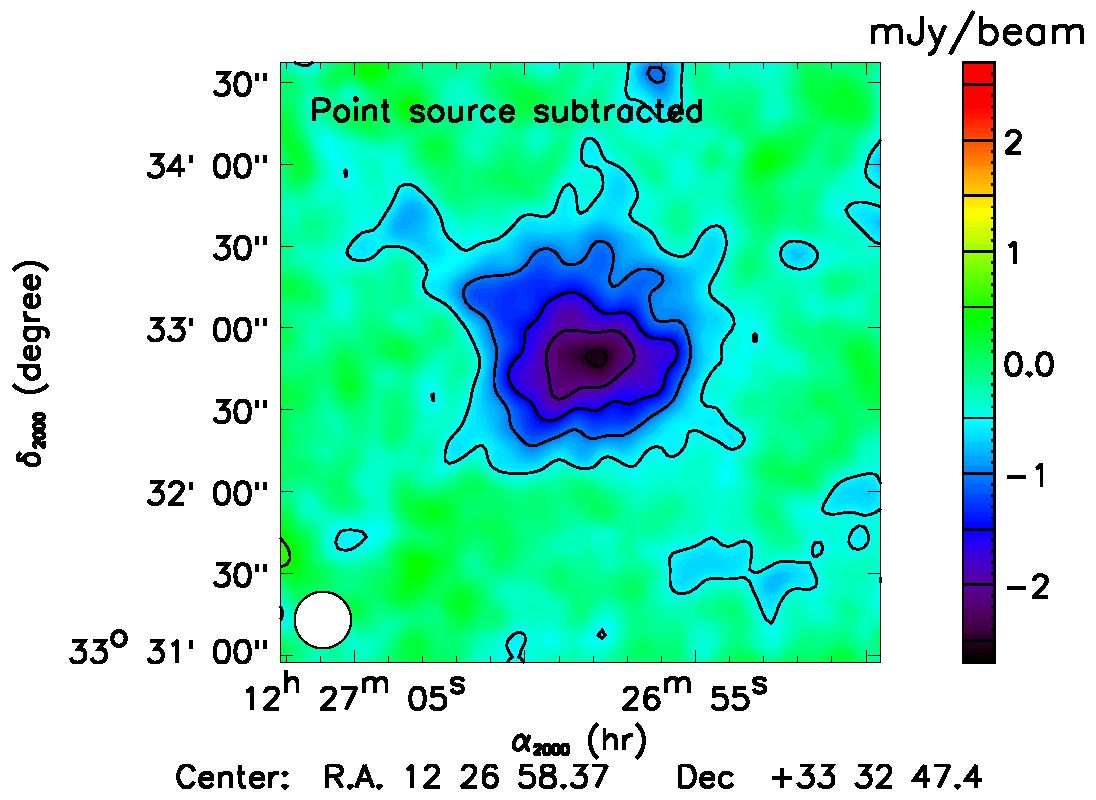
\includegraphics[width=0.47\columnwidth]{./Figures/CL1226.pdf}
   \includegraphics[width=0.49\columnwidth]{./Figures/NIKA2_cl_sample_y_withCL_xmm.eps}
\caption{{\small {\bf Left:} NIKA map of CL J1226.9+3332 at 150 GHz \citep[from][]{Adam2015}. The effective beam FWHM (18.2 arcsec native resolution plus an extra 10 arcsec FWHM Gaussian) is shown as the bottom left white circle.  The overall effective observing time on the cluster is 7.8 hours and $\theta_{500} \sim$ 2~arcmin for this cluster. {\bf Right:} Clusters extracted from the Planck and ACT (equatorial) tSZ-selected samples, in the redshift range we want to explore and observables from the Pico Veleta site (dec $>$ -11). As a function of redshift, we show the integrated tSZ signal (left) and the tSZ-estimated cluster total (right) mass of the sample of objects fulfilling our redshift ($>$ 0.5) and observability (dec $>$ -11) criteria. As a reference we show the high redshift cluster CL J1226.9+3332 and the Planck discovered PSZ1 G045.85+57.71, that have both been successfully observed by NIKA. The blue triangles represent the objects that have been already selected also for an on-going XMM large program (P.I.: M. Arnaud).}}
\label{Fig:CL_and_sample}
\end{figure}

\vspace{0.3cm} \noindent {\bf \large Sub-arcminute resolution tSZ observations with NIKA2 -- } 
%By contrast X-ray measurements are sensitive to the square of the gas density and the root square of the temperature. 
%We present in Figure 1 recent measurements of the stacked cluster radial pressure profile using tSZ observations with PLANCK, BOLOCAM and SPT and X-ray estimates. From the
%left plot we can notice that the tSZ measurements are in good agreement but are not able to sample the inner part of the clusters, which present a cool-core (CC), and disturbed ones (non-CC). This is more obvious 
The NIKA2 camera is particularly well adapted for high resolution observations of the tSZ effect from cluster of galaxies:
\begin{itemize}
\item [a)] It operates simultaneously at two frequency bands, 150 and 260 GHz, at which tSZ shows up as a negative and a positive distortion of the CMB spectrum, producing a very distinctive cluster signal on the observed maps. Dual-band observations can be used to remove the atmospheric noise without affecting the signal, taking advantage of the characteristic tSZ spectrum (and then recover both small  and large angular scales with the price of a worse sensitivity). In addition they are of the outmost interest to detect foreground contaminating sources, and account for their flux.
\item [b)] NIKA2 is made of arrays of thousands of high sensitive Kinetic Inductance Detectors (KIDs). In particular we expect a sensitivity in Compton parameter units of $\sim$~10$^{-4}$ per hour and per beam. This should allow us to obtain reliable tSZ detections and mapping of clusters of galaxies in few hours.
\item [c)] NIKA2, coupled to the IRAM 30 m telescope allows us to map clusters of galaxies to a resolution of typically 20 arcsec within a 6.5 arcmin diameter FOV. This is well adapted for medium and high redshift clusters for which we expect typical angular sizes of about 6-11 arcmin. %(Figure \ref{Fig:size}).
\end{itemize}

NIKA2 tSZ capabilities have been demonstrated through a pilot study conducted with its pathfinder, NIKA. In the context of this pilot study, in order to validate the KIDs capabilities when dealing with such a faint and diffuse signal, we have mapped the tSZ signal in the direction of six clusters of galaxies:  
{\bf i)} RX~J1347.5-1145, an intermediate redshift object (z=0.45), which is the perfect test target for the first tSZ detection ever achieved with KIDs \citep{Adam2014}; {\bf ii)} CL~J1226.9+3332, a very high redshift cluster \citep[z~$=$~0.89, ][the tSZ map at 150~GHz is shown in the left panel of Fig. \ref{Fig:CL_and_sample}]{Adam2015}, {\bf iii)} MACS~J0717.5+3745, characterized by a complex morphology \citep{Moriond2014}; {\bf iv)} MACS~J1423.9+2404 a relaxed cluster, which was used to explore the impact of the presence of foreground radio and IR sources and how to deal with them in the data reduction (Adam et al. in prep.); {\bf v)} PSZ1~G046.13+30.75 and PSZ1~G045.85+57.71, two newly Planck tSZ discovered clusters (at z=0.57 and z=0.61, respectively) chosen to test NIKA2 capabilities at the level of detection of the Planck catalogue of tSZ sources (NIKA Collaboration in prep.). We have successfully explored a wide range of cluster morphologies and amplitudes of the tSZ flux. \\
%\vspace{0.3cm} \noindent {\bf \large Comparison with other high-angular resolution tSZ facilities -- } 
%It is important to compare NIKA2 to other existing and planned instruments for high resolution tSZ observations. 
To date, the Mustang and Bolocam instruments (at the focus of the Green Bank Telescope and of the Caltech Submillimeter Observatory, respectively) have produced scientific quality tSZ observations \citep{Korngut2011, Mroczkowski2012, Young2014, Sayers2011, Sayers2013, Czakon2014}. They are expected to be followed by next generation instruments, Mustang-2 and BolocamII, which represent the closest NIKA2 concurrent experiences. However, none of them will be operational before NIKA2 and none of them will combine sufficiently large FOV and high angular resolution to attempt the project described here. As an alternative to large diameter telescopes, interferometers (e.g. CARMA) can reach very high angular resolution, but they cannot recover the large scale signal and they are time expensive. 

%Working at the focus of the Green Bank Telescope (GBT), Mustang has produced extremely interesting tSZ observations at 90 GHz \citep{Korngut2011, Mroczkowski2012, Young2014}. The system is in fact able to reach a 9 arcsec angular resolution, but with a relatively small instantaneous FOV (42 arcsec). Its characteristics will be improved by Mustang-2 \citep{Mustang2}, a large focal plane array (TES, transition edge sensor bolometers) for the 100 m Green Bank Telescope, that will have over 5 times the field-of-view and be over a factor of 5 times more sensitive with respect to Mustang. Installed at the Caltech Submillimeter Observatory (CSO) Bolocam provides, at 140 or 268 GHz, resolutions of 58'' and 31'', respectively, with an 8' FOV \citep{Sayers2011, Sayers2013, Czakon2014}. Working at the focus of the Large Millimeter Telescope (LMT, 50 m of diameter) BolocamII will result in a 2' field of view and approximately 6', 8', and 12' for the FWHM at 1.1mm, 1.4mm, and 2.1mm, respectively.

%None of these concurrent experiences will be operational before NIKA2, and none of them is conceived to produce dual band observations. 

%Previous works and programs dedicated to a similar goal have been conducted with Bolocam \citep{Sayers2013, Czakon2014}, SPT \citep{Plagge2010} and Planck \citep{PPP}. Planck (62 objects also observed by the X-ray mission XMM) and SPT samples are limited to the local universe (z $<$ 0.4), because of their relatively low angular resolution. The Bolocam sample is made up of 45 clusters (0.15 $<$ z $<$ 0.9, with a median redshift of 0.42). This sample is biased towards intermediate z because the selection criterion is mainly driven by the instrument resolution and FOV as well as by the requirement of having already existing complementary X-ray and optical data. Furthermore, they have selected clusters that have X-ray derived temperatures of the gas that are higher than the average, in order to ensure stronger tSZ brightnesses. The {\it ad hoc} nature of the selection strategy adopted implies a non-trivial selection function, that is specific to the Bolocam sample. Our selection strategy has been conceived to avoid this problem.

\vspace{0.3cm} \noindent {\bf Observing strategy and data reduction -- } 
Based on the experience with the NIKA camera, we will perform OnTheFly (OTF) scans in right ascension and declination. We will alternate different orientations of the scans (e.g. 0, 45, 90,-45 degrees) and perform scans of 13' $\times$ 8' (about one third of the observing time will be spent on the core of the signal) so that we reach cluster outskirts (roughly up to twice the characteristic radius of the cluster r$_{500}$) even for the lowest redshift clusters. This will allow us to properly define the zero level of the final map and measure angular scales structures up to the scan size. Smaller scans of 11' $\times$ 7' will be considered in the case of high redshift and low mass clusters ($\theta_{500}$ $<$ 2.25 arcmin). 

We take the Y$_{500}$ (Y$_{500} =  \int_{\Omega_{r_{500}}}y d\Omega$), M$_{500}$ and redshift from the latest updated version of PSZ1 and the ACT catalogs. We then consider an universal pressure profile \citep{Arnaud2010} to model the distribution of the signal around the cluster center for each given Y$_{500}$. The estimates of the required observation time are optimized cluster by cluster, in order to obtain an homogeneous sample in terms of signal to noise at a given characteristic radius (r$_{500}$). r$_{500}$ is computed from the redshift and the tSZ-derived M$_{500}$ reported in the catalogues, in order to have a homogeneous definition that only depends on the tSZ flux and the cluster distance.

To estimate the observing time needed per cluster we have performed simulations including signal, as just discussed, and noise. In terms of noise we have considered simulations taking the NIKA2 specification sensitivity at 2$~$mm of 20 mJy/beam/s$^{1/2}$
%(although we already know NIKA was about 10-15 mJy/beam/s$^{1/2}$)
, and increased the noise by 30 \% to account for correlated noise extra variance. In addition, we have considered the real FOV of the instrument (6.5') and a FWHM of 20'' at 2$~$mm. By contrast we have considered no atmospheric contamination and uniform weather conditions across the sample. 

As one of the major objectifs of the project is to have a clear picture of the morphology of the clusters we need to set strong requirements on the signal-to-noise at the map level to ensure structures
are significantly detected at least up to $\theta_{500}$. As we expect the SZ signal to peak towards the center of the cluster this criteria also ensure significant detection in the inner part of the cluster.
Assuming a perfect reconstruction of the cluster up to $\theta_{500}$ (no filtering) and requiring 4$~\sigma$ detection at $\theta_{500}$ on the map for pixels of the size of the beam, we can compute the needed observing time per cluster.  In addition we also impose a minimum of 1 hour of integration per cluster to ensure sufficient  scan redundancy.  If the final instrument performance are improved with respect to the specifications we plan to keep the same number of clusters as well as of the same observation time per cluster in order to recover large scale structures beyond $\theta_{500}$.

In terms of data reduction we will use the tSZ dedicated pipeline developed for the NIKA experiments. Needed improvements and updates will be directly carried out by our team.
%Depending on the depth in $Y_{500}$ (and in M$_{tot}$) that we want to reach, the observing time required can vary significantly. The total observing time can be significantly reduced if we decide to focus on radial profiles, since we gain a factor that is equal to the square root of the number of independent regions per annulus. However, given the goal of this project and the larger number of disturbed systems, deviating from the circular symmetry, expected at high-z, the choice of the observing time should aim at image the distribution of the projected tSZ signal within clusters. 

%To estimate the observing time needed per cluster we have performed simulations including noise and signal. In terms of noise we have considered realistic simulations taking the NIKA2 specification sensitivity of 20 mJy/beam/s$^{1/2}$ (although we already know NIKA was about 10-15 mJy/beam/s$^{1/2}$) and accounting for the real FOV of the instrument (6.5'). By contrast we have considered no atmospheric contamination and uniform weather conditions across the sample. The integrated tSZ fluxes reported in the Planck catalogue \citep{PSZ1} have been used to produce the expected tSZ maps with an \cite{Arnaud2010} model for the radial pressure profile. %We show in Figure 4 different cases for different values of integrated Ys. 
%Depending on the depth in $Y_{500}$ (and in M$_{tot}$) that we want to reach, the observing time required can vary significantly. Only 3h are needed to reach a 3? detection on the map at ? r500 for the cluster shown in the top-left panel, while 10h and a reduced 11' $\times$ 7' size of the map are required to obtain a map of the same quality at lower fluxes (middle panel, the plot shows the 10'  $\times$ 10' case). The total observing time can be significantly reduced if we decide to focus on radial profiles, since we gain a factor that is equal to the square root of the number of independent regions per annulus. However, given the goal of this project and the larger number of disturbed systems, deviating from the circular symmetry, expected at high-z, we think that the choice of the observing time should aim at image the distribution of the projected tSZ signal within clusters. A compromise is to be found.

\vspace{0.3cm} \noindent {\bf \large List of targets -- } 
The current status of the follow-up observations of tSZ discovered Planck clusters (not fully completed) does not allow us to present a definitive catalogue of clusters of galaxies. However, using the above criteria and the Planck and ACT samples we have pre-selected a first sample of clusters of galaxies suitable for our purposes. %(Tab. \ref{tab:ACT_sample} and \ref{tab:PSZ1_sample}). 
From the total sample we have performed a selection assuming {\bf two bins in redshift (0.5~$<$~z~$\le$~0.7 and 0.7~$<$~z~$\le$ 0.9)}.
For each interval in redshift, we have considered {\bf five bins in Y$_{500}$} (Fig. \ref{Fig:sample}). Within each bin we have selected five clusters randomly, giving preference to those that have been selected also for an on-going XMM large program (P.I.: M. Arnaud). We have limited our selection process to ACT and PSZ1 clusters but for two of them (selected from PSZ2), in order to reach the required number of five clusters in two of the boxes in the z~-~Y$_{500}$ plane (cyan triangles in Figure \ref{Fig:sample}). The systematic follow-up for confirmation and redshift determination has in fact been completed for PSZ1 but it is still on-going for PSZ2. So choosing clusters from the PSZ2 catalogue would bias our selection towards those for which the z information already exists. For the two largest Y$_{500}$ boxes of the high redshift bin we have at present only 4 and 0 clusters. Therefore we have selected only 44 clusters for a total of about 210 hours. The 6 remaining clusters will be defined later, since in the coming years follow-ups will further populate the z $>$ 0.6 region. We expect these 6 clusters to account for less than 10 hours of observing time. Then, in total, we will need 220 hours of on source observations. The selected clusters are given in Tab.~\ref{tab:z1_selected_sample}~and~\ref{tab:z2_selected_sample}. Finally, 50 hours will be dedicated to calibration. We have also reserved a total of 30 hours (10 \% of the total) for possible loss of data due to bad weather, for example.

%Of course we consider only clusters that are visible with the IRAM 30 m telescope. From this list we will do a random extraction for logarithmic interval in Y ($\propto M_{tot}$) in a way that reflects the relative abundances of clusters with a given mass at a given $z$. By the end of the summer an update of the PSZ1 will be produced. 

\vspace{0.3cm} \noindent {\bf \large Complementary external data -- } 
The scientific output of the NIKA2 LP could be enriched by the use of high quality external data at other wavelengths. Other than the use of publicly available data, formal collaborations are expected to be established to collect extra proprietary data. At this regard, XMM data from a companion X-ray follow up of high redshift clusters will be used.
With NIKA2 the cluster gas will be finally mapped in tSZ with a quality (in terms of sensitivity and angular resolution) comparable to X-ray, even for intermediate and high-redshift clusters. Then, the natural combination of these two direct observables of the intra-cluster hot gas (i.e., tSZ and X-ray measurements) will allow us to estimate the total masses (under the assumption of hydrostatic equilibrium) as well as a full physical characterization of the (radial) distribution of the cluster thermodynamic properties: not only pressure, but also temperature  (T$_{e}$(r) $\propto$ P$_{e}$(r)/n$_{e}$(r)) and entropy (K(r) $\propto$ P$_{e}$(r)n$_{e}^{-5/3}$) which are essential to unveil cluster thermodynamic history. Indeed, the tSZ signal directly probes the gas pressure, while X-ray data deliver the gas density squared and temperature. The different dependencies of tSZ and X on the electron density will also provide a powerful probe of gas clumping, and an improved insight on the cluster tridimensional shape. %Selecting only clusters that have been already observed in X-rays (by XMM or Chandra) would bias the cluster selection towards an X-ray selected sample. Furthermore, combining X-ray and tSZ provides access to the temperature information. Which implies that, for clusters that have not yet been observed in X, we will need to ask only relatively cheep (in terms of observation time) XMM snapshots. 
Furthermore, optical follow-ups could be performed for a large number of the NIKA2 clusters using the GTC (Gran Telescopio Canarias) imaging and spectroscopy facilities. The combination of tSZ and X-ray data to optical/NIR observations of the cluster galaxies will further help to investigate the connection between galaxy properties (luminosity function, SFR, stellar mass) and those of the ICM, and thereby bring constraints on feedback mechanisms at play within clusters. Moreover, weak lensing measurements will provide complementary measurements of the dark matter distribution and total mass of the clusters, in a totally independent way, then affected by different systematics. Optical mass estimate are not based on the same assumptions.


%With NIKA2 the cluster gas will be finally mapped in tSZ with a quality (in terms of sensitivity and angular resolution) comparable to X-ray, even for intermediate and high-redshift clusters. Then, the natural combination of direct observables of the intra-cluster hot gas (i.e., tSZ and X-ray measurements), as well as of the dark matter distribution (i.e, optical weak lensing measurements), will allow a full physical characterization of the (radial) distribution of the physical properties of clusters. %including pressure, entropy, gas mass, total mass, gas fraction and clumpiness of the gas. Indeed, the tSZ signal directly probes the gas pressure, while X-ray data deliver the gas density squared and temperature. The combination of the two observables is the only way to provided an unbiased estimate of the entropy and clumpiness of the gas: pressure profiles (P$_e$(r)) with spatial resolution comparable to those of X-ray derived electron densities (n$_e$(r)) can be used to study the cluster radial distribution of temperature  (T$_{e}$(r) $\propto$ P$_{e}$(r)/n$_{e}$(r)) and entropy (K(r) $\propto$ P$_{e}$(r)n$_{e}^{-5/3}$), which are essential to unveil cluster thermodynamic history. In addition, optical follow could be performed for a large number of the NIKA2 clusters using the GTC (Gran Telescopio Canarias) imaging and spectroscopy facilities. 

NIKA2 will be able to observe simultaneously at two wavelengths, and this represents a great advantage for foreground source subtraction \citep[][Adam \& NIKA collaboration in prep.]{Adam2015}. However PdBI, and its evolution into NOEMA (Northern Extended Millimetric Array project, 12 antennas with a diameter of 15 m, at 2550 m above the sea level), could be eventually used to obtain complementary information in this sense, requiring reasonable observing times.

%In addition, the IRAM 30 m telescope and PdBI (Plateau de Bure Interferometer) have produced complementary observations that are at the basis of several studies concerning the presence and distribution of molecular gas within and around the BCGs (brightest cluster galaxy, located at the center of clusters). Clusters are in fact at the crossroad of cosmology and astrophysics. And at present out limited knowledge of the astrophysical properties of the cluster population is what limits their cosmological exploitation.
%In order to understand the details of the evolution of the cluster population and its baryons, studies able to simultaneously investigate the hot, warm and cold baryonic component must be conducted. 
%A correlation between the ICM central cooling time (X) and the quantity of cold gas that could feed the BCG was in fact expected \citep[and observed, e.g.][]{Cavagnolo2008}. By combining single dish and interferometric observations several studies have been able to detect and analyse the presence and distribution of molecular clouds (e.g. through the presence of CO lines). Thanks to the high spatial resolution and sensitivity of ALMA and NOEMA, the number of clusters of galaxies for which this kind of study will be possible will be significantly enriched. And this will contribute to improve our understanding of the evolutionary history of these objects as well as the details of the different processes and interactions at play. Another interesting aspect is in the context of the introduction and validation of indicators of clusters morphology, and their possible correlation with deviation from the self-similar average behavior.

\vspace{0.3cm} \noindent {\bf \large Project management -- } 
For this project we have gathered a highly experienced team with a large expertise in sub millimetre observations, data reduction and tSZ science as well as complementary external observations.
A project PI and two co-PIs will coordinate the different activities: data reduction (mainly former NIKA tSZ team), analysis and interpretation (former NIKA and Planck collaboration tSZ experts), and
external ancillary data (XMM group for X-rays, LOFAR team for radio emission and GTC team for optical observations).

\vspace{0.3cm} \noindent {\bf \large Data policy -- } 
The project data and products will be made publicly available by the NIKA2 collaboration in a dedicated database, following the standard IRAM rules.


%\begin{table}
%\centering
%\begin{tabular}{|l  || c | c | c | c | c | c | }
 % \hline                       
%name  &  R.A.  & dec  &   z  & $\theta_{500}$ [arcmin] & Y$_{500}$ $\times$ 10$^{-4}$ [arcmin$^{2}$] & t$_{obs}$ [hr] \\ \hline
%   ACTCLJ0014.9-0057 & 3.728 & -0.950 & 0.533 & 2.8 & 5.0 & 4.7 \\ \hline
%   ACTCLJ0026.2+0120 & 6.570 & 1.337 & 0.650 & 2.2 & 2.8 & 5.1 \\ \hline
 %  ACTCLJ0045.2-0152 & 11.305 & -1.883 & 0.545 & 2.8 & 4.8 & 5.0 \\ \hline
 %  ACTCLJ0051.1+0055 & 12.788 & 0.932 & 0.690 & 1.7 & 0.9 & 21.8 \\ \hline
%   ACTCLJ0206.2-0114 & 31.557 & -1.243 & 0.676 & 2.2 & 2.6 & 5.7 \\ \hline
%   ACTCLJ0218.2-0041 & 34.563 & -0.688 & 0.672 & 2.1 & 2.2 & 7.6 \\ \hline
 %  ACTCLJ0219.8+0022 & 34.953 & 0.375 & 0.537 & 2.2 & 1.7 & 21.4 \\ \hline
 %  ACTCLJ0221.5-0012 & 35.393 & -0.206 & 0.589 & 1.6 & 0.5 & 67.2 \\ \hline
 %  ACTCLJ0223.1-0056 & 35.794 & -0.947 & 0.663 & 2.1 & 2.2 & 7.7 \\ \hline
%   5A5CTCLJ0240.0+0116 & 40.010 & 1.269 & 0.620 & 2.1 & 1.8 & 11.5 \\ \hline
%   ACTCLJ0241.2-0018 & 40.313 & -0.311 & 0.684 & 1.8 & 1.1 & 15.5 \\ \hline
%   ACTCLJ0301.1-0110 & 45.292 & -1.172 & 0.530 & 2.0 & 1.1 & 29.8 \\ \hline
 %  ACTCLJ0308.1+0103 & 47.048 & 1.061 & 0.633 & 1.9 & 1.3 & 19.9 \\ \hline
 %  ACTCLJ2050.5-0055 & 312.626 & -0.931 & 0.622 & 2.2 & 2.2 & 8.1 \\ \hline
%   ACTCLJ2152.9-0114 & 328.237 & -1.246 & 0.690 & 1.9 & 1.5 & 9.0 \\ \hline
 %  ACTCLJ2220.7-0042 & 335.192 & -0.710 & 0.570 & 2.0 & 1.2 & 24.7 \\ \hline
 %  ACTCLJ2229.2-0004 & 337.304 & -0.074 & 0.610 & 2.0 & 1.3 & 20.5 \\ \hline
%   ACTCLJ2253.3-0031 & 343.343 & -0.528 & 0.540 & 2.1 & 1.5 & 17.2 \\ \hline
%   ACTCLJ2302.5+0002 & 345.643 & 0.042 & 0.520 & 2.5 & 2.5 & 11.1 \\ \hline
 %  ACTCLJ0018.2-0022 & 4.562 & -0.380 & 0.750 & 1.8 & 1.5 & 8.4 \\ \hline
  % ACTCLJ0022.2-0036 & 5.555 & -0.605 & 0.805 & 2.1 & 3.8 & 2.5 \\ \hline
 %  ACTCLJ0058.0+0030 & 14.519 & 0.511 & 0.760 & 1.8 & 1.5 & 8.5 \\ \hline
  % ACTCLJ0059.1-0049 & 14.785 & -0.833 & 0.786 & 2.1 & 3.5 & 3.0 \\ \hline
 %  ACTCLJ0119.9+0055 & 19.997 & 0.919 & 0.720 & 1.9 & 1.7 & 7.0 \\ \hline
 %  ACTCLJ0139.3-0128 & 24.841 & -1.477 & 0.700 & 1.6 & 0.8 & 26.7 \\ \hline
 %  ACTCLJ0215.4+0030 & 33.870 & 0.509 & 0.865 & 1.9 & 1.8 & 5.5 \\ \hline
  % ACTCLJ0228.5+0030 & 37.125 & 0.503 & 0.720 & 1.7 & 1.0 & 17.7 \\ \hline
  % ACTCLJ0250.1+0008 & 42.537 & 0.140 & 0.780 & 1.7 & 1.2 & 12.0 \\ \hline
  % ACTCLJ2130.1+0045 & 322.537 & 0.759 & 0.710 & 1.9 & 1.6 & 7.9 \\ \hline
  % ACTCLJ0342.0+0105 & 55.501 & 1.087 & 1.070 & 1.5 & 1.8 & 2.7 \\ \hline
  % ACTCLJ2351.7+0009 & 357.935 & 0.154 & 0.990 & 1.5 & 1.5 & 3.9 \\ \hline
   %ACTCLJ0044.4+0113 & 11.108 & 1.222 & 1.110 & 1.3 & 1.1 & 6.2 \\ \hline
%\end{tabular}
 %\caption{{\small ACT sample of tSZ-selected clusters of galaxies in the redshift range we want to explore (z $>$ 0.5) and observable from the Pico Veleta site (dec $>$ -11).}}
 %\label{tab:ACT_sample}
%\end{table}

%\begin{table}
%\centering
%\begin{tabular}{|l  || c | c | c | c | c | c | }
 % \hline                       
%name  &  R.A.  & dec  &   z  & $\theta_{500}$ [arcmin] & Y$_{500}$ $\times$ 10$^{-4}$ [arcmin$^{2}$] & t$_{obs}$ [hr] \\ \hline
 % PSZ1 G024.20+19.61 & 261.513 & 1.480 & 0.651 & 2.623 & 7.946 & 1.8 \\ \hline
 % PSZ1 G045.18-36.47 & 320.538 & -6.843 & 0.534 & 2.886 & 7.228 & 3.6 \\ \hline
 % PSZ1 G045.85+57.71 & 229.580 & 29.457 & 0.611 & 2.737 & 8.212 & 1.8 \\ \hline
 % PSZ1 G046.13+30.75 & 259.251 & 24.074 & 0.569 & 2.818 & 7.710 & 2.1 \\ \hline
 % PSZ1 G058.82-49.66 & 337.058 & -5.511 & 0.520 & 2.865 & 6.381 & 4.5 \\ \hline
 % PSZ1 G066.41+27.03 & 269.201 & 40.133 & 0.576 & 2.790 & 7.576 & 2.2 \\ \hline
 % PSZ1 G070.91+49.26 & 239.179 & 44.661 & 0.604 & 2.561 & 5.544 & 3.6 \\ \hline
 %PSZ1 G073.22+67.57 & 215.136 & 39.870 & 0.609 & 2.311 & 3.276 & 6.2 \\ \hline
 % PSZ1 G073.64+36.49 & 257.387 & 47.553 & 0.560 & 2.688 & 5.688 & 3.6 \\ \hline
 % PSZ1 G086.93+53.18 & 228.487 & 52.797 & 0.675 & 2.255 & 3.961 & 4.1 \\ \hline
  %PSZ1 G094.54+51.01 & 227.104 & 57.889 & 0.539 & 2.656 & 4.757 & 5.1 \\ \hline
 % PSZ1 G099.84+58.45 & 213.700 & 54.778 & 0.631 & 2.516 & 5.759 & 3.3 \\ \hline
 % PSZ1 G102.86-31.07 & 353.283 & 28.731 & 0.591 & 2.837 & 8.988 & 2.3 \\ \hline
 % PSZ1 G104.78+40.45 & 236.593 & 69.950 & 0.690 & 2.171 & 3.453 & 5.2 \\ \hline
 % PSZ1 G106.15+25.76 & 284.252 & 74.928 & 0.588 & 2.486 & 4.351 & 3.9 \\ \hline
 % PSZ1 G108.26+48.66 & 216.797 & 65.650 & 0.674 & 2.193 & 3.390 & 5.4 \\ \hline
 % PSZ1 G109.49-45.40 & 3.067 & 16.443 & 0.534 & 2.857 & 6.830 & 3.9 \\ \hline
 % PSZ1 G111.60-45.72 & 4.644 & 16.426 & 0.546 & 3.056 & 10.457 & 1.8 \\ \hline
 % PSZ1 G127.02+26.21 & 89.847 & 86.228 & 0.630 & 2.599 & 6.843 & 2.4 \\ \hline
 % PSZ1 G135.24+65.43 & 184.777 & 50.913 & 0.527 & 2.852 & 6.502 & 4.3 \\ \hline
 % PSZ1 G144.86+25.09 & 101.919 & 70.223 & 0.584 & 2.775 & 7.680 & 2.1 \\ \hline
  %PSZ1 G147.86+53.24 & 164.412 & 58.024 & 0.600 & 2.544 & 5.242 & 4.0 \\ \hline
 % %PSZ1 G153.41+36.58 & 130.667 & 62.575 & 0.650 & NaN & NaN & NaN \\ \hline
  %PSZ1 G155.25-68.42 & 24.328 & -8.478 & 0.566 & 3.019 & 10.951 & 1.6 \\ \hline
  %PSZ1 G159.26+71.11 & 178.010 & 41.565 & 0.533 & 2.837 & 6.529 & 4.3 \\ \hline
  %PSZ1 G171.01+39.44 & 132.748 & 48.491 & 0.554 & 3.015 & 10.165 & 1.9 \\ \hline
  %PSZ1 G180.00+51.58 & 149.025 & 41.136 & 0.587 & 2.699 & 6.728 & 2.6 \\ \hline
  %PSZ1 G180.25+21.03 & 109.367 & 37.743 & 0.546 & 3.329 & 16.605 & 1.1 \\ \hline
  %PSZ1 G183.92+42.99 & 137.697 & 38.803 & 0.561 & 2.735 & 6.281 & 3.1 \\ \hline
  %PSZ1 G193.29-46.13 & 53.968 & -6.977 & 0.640 & 2.515 & 6.018 & 3.0 \\ \hline
  %PSZ1 G199.71+46.53 & 143.472 & 28.095 & 0.553 & 2.751 & 6.211 & 3.2 \\ \hline
  %PSZ1 G201.50-27.34 & 73.533 & -3.034 & 0.538 & 2.905 & 7.616 & 3.2 \\ \hline
  %PSZ1 G209.80+10.23 & 110.608 & 7.396 & 0.677 & 2.613 & 8.792 & 1.5 \\ \hline
  %PSZ1 G211.23+38.63 & 137.785 & 17.774 & 0.505 & 2.919 & 6.456 & 4.5 \\ \hline
  %PSZ1 G212.51+63.18 & 163.225 & 24.197 & 0.550 & 2.772 & 6.361 & 3.0 \\ \hline
  %PSZ1 G213.37+80.60 & 182.338 & 26.664 & 0.559 & 2.804 & 7.086 & 2.5 \\ \hline
  %PSZ1 G228.21+75.20 & 177.406 & 22.393 & 0.545 & 3.043 & 10.201 & 1.9 \\ \hline
  %PSZ1 G229.08+16.09 & 124.633 & -6.405 & 0.512 & 2.898 & 6.486 & 4.4 \\ \hline
  %PSZ1 G236.86+66.33 & 170.445 & 15.829 & 0.559 & 2.722 & 6.068 & 3.3 \\ \hline
  %PSZ1 G282.30+49.92 & 179.509 & -10.799 & 0.660 & 2.484 & 6.199 & 1.9 \\ \hline
  %PSZ1 G048.09+27.18 & 263.565 & 24.544 & 0.736 & 2.355 & 6.553 & 1.6 \\ \hline
  %PSZ1 G065.13+57.53 & 229.067 & 39.744 & 0.720 & 2.295 & 5.322 & 2.3 \\ \hline
  %PSZ1 G080.66-57.87 & 351.890 & -2.062 & 0.705 & 2.518 & 8.182 & 1.6 \\ \hline
  %PSZ1 G084.04+58.75 & 222.307 & 48.522 & 0.731 & 2.213 & 4.586 & 3.0 \\ \hline
  %PSZ1 G089.04+55.07 & 224.752 & 52.827 & 0.702 & 2.215 & 4.071 & 3.8 \\ \hline
  %PSZ1 G091.82+26.11 & 277.784 & 62.248 & 0.822 & 2.192 & 6.306 & 1.6 \\ \hline
  %PSZ1 G138.60-10.85 & 36.756 & 49.082 & 0.702 & 2.618 & 9.669 & 1.2 \\ \hline
  %PSZ1 G141.73+14.22 & 70.257 & 68.235 & 0.830 & 2.209 & 6.789 & 1.4 \\ \hline
  %PSZ1 G183.26+12.25 & 100.732 & 31.819 & 0.850 & 2.226 & 7.637 & 1.1 \\ \hline
  %PSZ1 G224.73+33.65 & 137.876 & 5.807 & 0.768 & 2.303 & 6.647 & 1.5 \\ \hline
  %PSZ1 G226.65+28.43 & 134.131 & 1.803 & 0.724 & 2.190 & 4.209 & 3.5 \\ \hline
  %\end{tabular}
 %\caption{{\small PSZ1 confirmed cluster sample in the redshift range we want to explore (z $>$ 0.5) and observable from the Pico Veleta site (dec $>$ -11).}}
 %\label{tab:PSZ1_sample}
%\end{table}

\begin{table}
\centering
\begin{tabular}{|l  || c  | c | c | c | c | }
  \hline                       
name  &   z  & $\theta_{500}$ [arcmin] & Y$_{500}$ $\times$ 10$^{-4}$ [arcmin$^{2}$] & t$_{obs}$ [hr] \\ \hline
   ACTCLJ0241.2-0018  & 0.684 & 1.723 & 1.100 & 15.5 \\ \hline
   ACTCLJ0219.8+0022  & 0.537 & 2.169 & 1.700 & 21.4 \\ \hline
   ACTCLJ0240.0+0116  & 0.620 & 2.022 & 1.800 & 11.5 \\ \hline
   ACTCLJ0218.2-0041  & 0.672 & 2.005 & 2.200 & 7.6 \\ \hline
   ACTCLJ2050.5-0055  & 0.622 & 2.115 & 2.200 & 8.1 \\ \hline
  PSZ1 G073.22+67.57  & 0.609 & 2.311 & 3.276 & 6.2 \\ \hline
  PSZ1 G104.78+40.45  & 0.690 & 2.171 & 3.453 & 5.2 \\ \hline
  PSZ1 G086.93+53.18  & 0.675 & 2.255 & 3.961 & 4.1 \\ \hline
  PSZ1 G106.15+25.76  & 0.588 & 2.486 & 4.351 & 3.9 \\ \hline
  PSZ1 G094.54+51.01  & 0.539 & 2.656 & 4.757 & 5.1 \\ \hline
  PSZ1 G147.86+53.24  & 0.600 & 2.544 & 5.242 & 4.0 \\ \hline
  PSZ1 G070.91+49.26  & 0.604 & 2.561 & 5.544 & 3.6 \\ \hline
  PSZ1 G193.29-46.13  & 0.640 & 2.515 & 6.018 & 3.0 \\ \hline
  PSZ1 G183.92+42.99  & 0.561 & 2.735 & 6.281 & 3.1 \\ \hline
  PSZ1 G211.23+38.63  & 0.505 & 2.919 & 6.456 & 4.5 \\ \hline
  PSZ1 G201.50-27.34  & 0.538 & 2.905 & 7.616 & 3.2 \\ \hline
  PSZ1 G144.86+25.09  & 0.584 & 2.775 & 7.680 & 2.1 \\ \hline
  PSZ1 G046.13+30.75  & 0.569 & 2.818 & 7.710 & 2.1 \\ \hline
  PSZ1 G209.80+10.23  & 0.677 & 2.613 & 8.792 & 1.5 \\ \hline
  PSZ1 G102.86-31.07  & 0.591 & 2.837 & 8.988 & 2.3 \\ \hline
  PSZ1 G171.01+39.44  & 0.554 & 3.015 & 10.165 & 1.9 \\ \hline 
  PSZ1 G228.21+75.20  & 0.545 & 3.043 & 10.201 & 1.9 \\ \hline
  PSZ1 G111.60-45.72  & 0.546 & 3.056 & 10.457 & 1.8 \\ \hline
  PSZ1 G155.25-68.42  & 0.566 & 3.019 & 10.951 & 1.6 \\ \hline
  PSZ2 G128.18-51.08  & 0.546 & 2.788 & 13.553 & 1.0 \\ \hline
\end{tabular}
 \caption{{\small 0.5 $\leq$ z $<$ 0.7 selected sample: 25 clusters.}}
\label{tab:z1_selected_sample}
\end{table}

\begin{table}
\centering
\begin{tabular}{|l  || c  | c | c | c | c | }
  \hline                       
name  &   z  & $\theta_{500}$ [arcmin] & Y$_{500}$ $\times$ 10$^{-4}$ [arcmin$^{2}$] & t$_{obs}$ [hr] \\ \hline
   ACTCLJ0228.5+0030 & 0.720 & 1.641 & 1.000 & 17.7 \\ \hline
   ACTCLJ0250.1+0008 & 0.780 & 1.618 & 1.200 & 12.0 \\ \hline
   ACTCLJ0018.2-0022 & 0.750 & 1.739 & 1.500 & 8.4 \\ \hline
   ACTCLJ0058.0+0030 & 0.760 & 1.742 & 1.500 & 8.5 \\ \hline
   ACTCLJ0215.4+0030 & 0.865 & 1.648 & 1.800 & 5.5 \\ \hline
   ACTCLJ0059.1-0049 & 0.786 & 2.002 & 3.500 & 3.0 \\ \hline
   ACTCLJ0022.2-0036 & 0.805 & 2.008 & 3.800 & 2.5 \\ \hline
  PSZ1 G089.04+55.07 & 0.702 & 2.215 & 4.071 & 3.8 \\ \hline
  PSZ1 G226.65+28.43 & 0.724 & 2.190 & 4.209 & 3.5 \\ \hline
  PSZ1 G084.04+58.75 & 0.731 & 2.213 & 4.586 & 3.0 \\ \hline
  PSZ1 G065.13+57.53 & 0.720 & 2.295 & 5.322 & 2.3 \\ \hline
  PSZ1 G091.82+26.11 & 0.822 & 2.192 & 6.306 & 1.6 \\ \hline
  PSZ1 G048.09+27.18 & 0.736 & 2.355 & 6.553 & 1.6 \\ \hline
  PSZ1 G224.73+33.65 & 0.768 & 2.303 & 6.647 & 1.5 \\ \hline
  PSZ1 G141.73+14.22 & 0.830 & 2.209 & 6.789 & 1.4 \\ \hline
  PSZ1 G183.26+12.25 & 0.850 & 2.226 & 7.637 & 1.1 \\ \hline
  PSZ1 G080.66-57.87 & 0.705 & 2.518 & 8.182 & 1.6 \\ \hline
  PSZ2 G160.83+81.66 & 0.888 & 1.907 & 9.043 & 1.0 \\ \hline
  PSZ1 G138.60-10.85 & 0.702 & 2.618 & 9.669 & 1.2 \\ \hline
  \hline
\end{tabular}
 \caption{{\small 0.7 $\leq$ z $<$ 0.9 selected sample.}}
 \label{tab:z2_selected_sample}
\end{table}

\begin{figure}
  \centering
   \includegraphics[width=0.8\columnwidth]{./Figures/NIKA2_selected_sample_y_withCL_xmm.eps}
\caption{{\small Selected sample of 44 clusters extracted from the Planck and ACT (equatorial) tSZ-selected cluster catalogues, selected from those fulfilling our redshift ($>$ 0.5) and observability (dec $>$ -11) criteria. The selected objects are shown in the Y$_{500}$ - z plane.}} %As a reference we show the high redshift cluster CL J1226.9+3332 and the Planck discovered PSZ1 G045.85+57.71, that have both been successfully observed by NIKA.}
\label{Fig:sample}
\end{figure}


% Bibliography and bibfile
\def\aj{AJ}%
          % Astronomical Journal
\def\actaa{Acta Astron.}%
          % Acta Astronomica
\def\araa{ARA\&A}%
          % Annual Review of Astron and Astrophys
\def\apj{ApJ}%
          % Astrophysical Journal
\def\apjl{ApJ}%
          % Astrophysical Journal, Letters
\def\apjs{ApJS}%
          % Astrophysical Journal, Supplement
\def\ao{Appl.~Opt.}%
          % Applied Optics
\def\apss{Ap\&SS}%
          % Astrophysics and Space Science
\def\aap{A\&A}%
          % Astronomy and Astrophysics
\def\aapr{A\&A~Rev.}%
          % Astronomy and Astrophysics Reviews
\def\aaps{A\&AS}%
          % Astronomy and Astrophysics, Supplement
\def\azh{AZh}%
          % Astronomicheskii Zhurnal
\def\baas{BAAS}%
          % Bulletin of the AAS
\def\bac{Bull. astr. Inst. Czechosl.}%
          % Bulletin of the Astronomical Institutes of Czechoslovakia 
\def\caa{Chinese Astron. Astrophys.}%
          % Chinese Astronomy and Astrophysics
\def\cjaa{Chinese J. Astron. Astrophys.}%
          % Chinese Journal of Astronomy and Astrophysics
\def\icarus{Icarus}%
          % Icarus
\def\jcap{J. Cosmology Astropart. Phys.}%
          % Journal of Cosmology and Astroparticle Physics
\def\jrasc{JRASC}%
          % Journal of the RAS of Canada
\def\mnras{MNRAS}%
          % Monthly Notices of the RAS
\def\memras{MmRAS}%
          % Memoirs of the RAS
\def\na{New A}%
          % New Astronomy
\def\nar{New A Rev.}%
          % New Astronomy Review
\def\pasa{PASA}%
          % Publications of the Astron. Soc. of Australia
\def\pra{Phys.~Rev.~A}%
          % Physical Review A: General Physics
\def\prb{Phys.~Rev.~B}%
          % Physical Review B: Solid State
\def\prc{Phys.~Rev.~C}%
          % Physical Review C
\def\prd{Phys.~Rev.~D}%
          % Physical Review D
\def\pre{Phys.~Rev.~E}%
          % Physical Review E
\def\prl{Phys.~Rev.~Lett.}%
          % Physical Review Letters
\def\pasp{PASP}%
          % Publications of the ASP
\def\pasj{PASJ}%
          % Publications of the ASJ
\def\qjras{QJRAS}%
          % Quarterly Journal of the RAS
\def\rmxaa{Rev. Mexicana Astron. Astrofis.}%
          % Revista Mexicana de Astronomia y Astrofisica
\def\skytel{S\&T}%
          % Sky and Telescope
\def\solphys{Sol.~Phys.}%
          % Solar Physics
\def\sovast{Soviet~Ast.}%
          % Soviet Astronomy
\def\ssr{Space~Sci.~Rev.}%
          % Space Science Reviews
\def\zap{ZAp}%
          % Zeitschrift fuer Astrophysik
\def\nat{Nature}%
          % Nature
\def\iaucirc{IAU~Circ.}%
          % IAU Cirulars
\def\aplett{Astrophys.~Lett.}%
          % Astrophysics Letters
\def\apspr{Astrophys.~Space~Phys.~Res.}%
          % Astrophysics Space Physics Research
\def\bain{Bull.~Astron.~Inst.~Netherlands}%
          % Bulletin Astronomical Institute of the Netherlands
\def\fcp{Fund.~Cosmic~Phys.}%
          % Fundamental Cosmic Physics
\def\gca{Geochim.~Cosmochim.~Acta}%
          % Geochimica Cosmochimica Acta
\def\grl{Geophys.~Res.~Lett.}%
          % Geophysics Research Letters
\def\jcp{J.~Chem.~Phys.}%
          % Journal of Chemical Physics
\def\jgr{J.~Geophys.~Res.}%
          % Journal of Geophysics Research
\def\jqsrt{J.~Quant.~Spec.~Radiat.~Transf.}%
          % Journal of Quantitiative Spectroscopy and Radiative Trasfer
\def\memsai{Mem.~Soc.~Astron.~Italiana}%
          % Mem. Societa Astronomica Italiana
\def\nphysa{Nucl.~Phys.~A}%
          % Nuclear Physics A
\def\physrep{Phys.~Rep.}%
          % Physics Reports
\def\physscr{Phys.~Scr}%
          % Physica Scripta
\def\planss{Planet.~Space~Sci.}%
          % Planetary Space Science
\def\procspie{Proc.~SPIE}%
          % Proceedings of the SPIE
\let\astap=\aap
\let\apjlett=\apjl
\let\apjsupp=\apjs
\let\applopt=\ao

\bibliography{biblio}



\end{document}
